\documentclass[10pt, a4paper, oneside]{ctexart}
\usepackage{amsmath, amsthm, amssymb, bm, ctex, graphicx, hyperref, mathrsfs, geometry, listings}

\usepackage[dvipsnames]{xcolor}
% 在导言区进行样式设置
\lstset{
    language=Python, % 设置语言
 basicstyle=\ttfamily, % 设置字体族
 breaklines=true, % 自动换行
 keywordstyle=\bfseries\color{NavyBlue}, % 设置关键字为粗体,颜色为 NavyBlue
 morekeywords={}, % 设置更多的关键字,用逗号分隔
 emph={self}, % 指定强调词,如果有多个,用逗号隔开
    emphstyle=\bfseries\color{Rhodamine}, % 强调词样式设置
    commentstyle=\itshape\color{black!50!white}, % 设置注释样式,斜体,浅灰色
    stringstyle=\bfseries\color{PineGreen!90!black}, % 设置字符串样式
    columns=flexible,
    numbers=left, % 显示行号在左边
    numbersep=2em, % 设置行号的具体位置
    numberstyle=\footnotesize, % 缩小行号
    frame=single, % 边框
    framesep=1em % 设置代码与边框的距离
}

\geometry{scale = 0.8}
\title{\textbf{计算概论第一次课程作业}}
\author{胡凯翔}
\date{\today}
\linespread{1.5}
\newcounter{problemname}
\newenvironment{problem}{\stepcounter{problemname}\par\noindent\textbf{题目\arabic{problemname}. }}{\\\par}
\newenvironment{solution}{\par\noindent\textbf{解答. }}{\\\par}
\newenvironment{note}{\par\noindent\textbf{题目\arabic{problemname}的注记. }}{\\\par}

\begin{document}

\maketitle

\begin{problem}
    \textbf{两篇文章总结}

\end{problem}

\begin{solution}

    The Great Principles of Computing

    在这篇有关计算科学文章中,作者Peter J.Denning主要阐述了计算作为一门独立科学领域的 演变与核心框架。首先,文章指出,计算始于20实际30年代哥德尔、图灵等人的数学几乎研究,早期被视为数学或工程的附属工具,但随着计算机的诞生及其在二战中的突破性应用(破解恩尼格玛密码),计算机逐渐发展为一个涵盖算法、网络、人工智能等多维度的学科。接着,文章指出,计算不仅时技术工具,更是继物理、生命和社会科学后的“第四大科学领域 ”,其本质在于研究自然与人工信息过程的转化与交互。通过七大核心原则——计算(可计算性)、通信(信息传输)、协调(多系统协作)、回忆(信息存储与检索)、自动化(算法设计)、评估(性能预测)和设计(系统可靠性)——计算科学构建了独特的理论框架,这些原则既独立又相互渗透,支撑着从芯片到互联网的复杂技术体系。之后,文章进一步强调,计算与物理、生命及社会科学深度交互:在物理领域,计算通过量子技术实现新范式;在生物学中,DNA翻译被视为自然信息过程;在社会领域,计算重塑人类协作与认知模式。同时,计算思维(将问题抽象为信息过程并寻求算法解)成为跨学科研究的通用方法论,推动了科学发现与技术革新。最终,作者指出,计算的核心价值在于其普适性——它不仅是工具,更是理解世界的新视角,其原则与互动模式揭示了信息过程在自然与人工系统中的根本作用,奠定了计算作为现代科学基石的不可替代地位。

    Computational thinking and thinking about computing

    本文由Jeannette M. Wing撰写,详细探讨了计算思维的定义、应用及其在教育中的重要性。首先,作者指出,计算思维是一种借鉴计算机科学基本概念的思考方法,涉及解决问题、设计系统和理解人类行为。计算思维通过抽象化将复杂问题简化,从而帮助人们更高效地处理海量数据、设计复杂系统以及解决传统方法无法解决的问题。具体而言,计算思维强调抽象化、模式识别、算法设计和自动化等核心元素,它不仅仅限于计算机操作,而是更广泛地应用于各个领域,改变了我们解决问题的方式。接着,作者介绍了计算思维在各学科领域中的深远影响。作者指出,计算思维已逐渐成为各学科的基础思维方式,特别是在科学、工程、经济学和生物学等领域。计算思维不仅在研究中提供新的视角和方法,也在实际应用中发挥着重要作用。例如,在生物学中,计算思维帮助科学家加速了基因组的测序;在经济学中,计算思维推动了计算微观经济学的发展,帮助解决诸如广告投放、在线拍卖和器官捐赠匹配等问题。因此,计算思维的普及已不再局限于计算机科学领域,而是扩展到社会各个层面,成为理解和解决当今复杂问题的重要工具。然后,文章说明,计算思维的普及面临着巨大的教育挑战,尤其是在如何有效地将其融入到教育体系中。作者指出,尽管许多大学和研究机构已经将计算思维纳入了课程内容,但基础教育阶段的普及仍然是一个重要的任务。为了确保每个学生都能够掌握计算思维,教育者需要思考如何在不同年龄阶段设计合理的教学方案。同时,作者还强调,计算思维的教学不仅仅是学习如何使用计算机工具,更重要的是要让学生理解背后的核心概念,如抽象化、自动化和算法设计等。作者认为,计算思维的学习不应仅仅停留在技术操作层面,而应深入到学生的思维方式和解决问题的能力中。最后,作者展望了计算思维在未来的发展趋势,并表明,计算思维将成为各行各业创新和发现的关键驱动力。随着计算技术的不断发展,尤其是量子计算、纳米计算和生物计算等前沿技术的突破,计算思维将迎来更加广阔的应用空间。此外,作者指出,计算思维的发展不仅受到科学和技术进步的推动,还与社会需求密切相关。例如,社会对更高效、更智能的计算机系统的需求,促使计算思维在各行各业得到广泛应用。总之,作者认为,计算思维将不仅仅是科技人员的专属工具,它将成为整个社会、整个教育体系和未来创新的重要基础。
\end{solution}

\begin{problem}
    为什么说计算思维的核心是“构造”,而构造的任务是抽象与自动化?你可以用身边的例子举例说明什么是计算思维吗?

\end{problem}

\begin{solution}
    
    计算思维的核心在于“构造”,其有助于有效地解决问题,而其任务主要包括抽象和自动化。
    抽象是指从复杂的现实问题中提取出关键特征,忽略不相关的细节,以便更好地建立模型和形式表示,而且需要支持机械地、一步步地自动执行,需要在抽象过程中进行精确和严格地符号标记和建模。自动化则是将这些抽象的解决方案转化为可由计算机执行的指令,实现高效、精确的处理。

    举例:假如我们要做一个有关大学生睡眠质量的课题,首先我们便要建立合理的评估模型,影响睡眠质量的因素有很多,要舍弃一些非常规的
    因素,着重聚焦于如入睡时间、睡前做了什么事、睡眠时间、精神压力等,将其量化;之后通过自动化,设计评估算法,不断与个人感觉的睡眠质量作比较,不断优化权重;最终经过大量数据的统计,便可找到权重高的
    影响因素,并得出最终结论。
\end{solution}

\begin{problem}
    请注册一个开源代码分享平台(如github、gitee) 维护个人资料(照片、自我介绍等)并上传一个代码。 将账号网站上传思源平台。

\end{problem}

\begin{solution}

    \href{https://github.com/kaxianghu}{github个人主页(https://github.com/kaxianghu)}

    \begin{figure}[htbp]
        \centering
        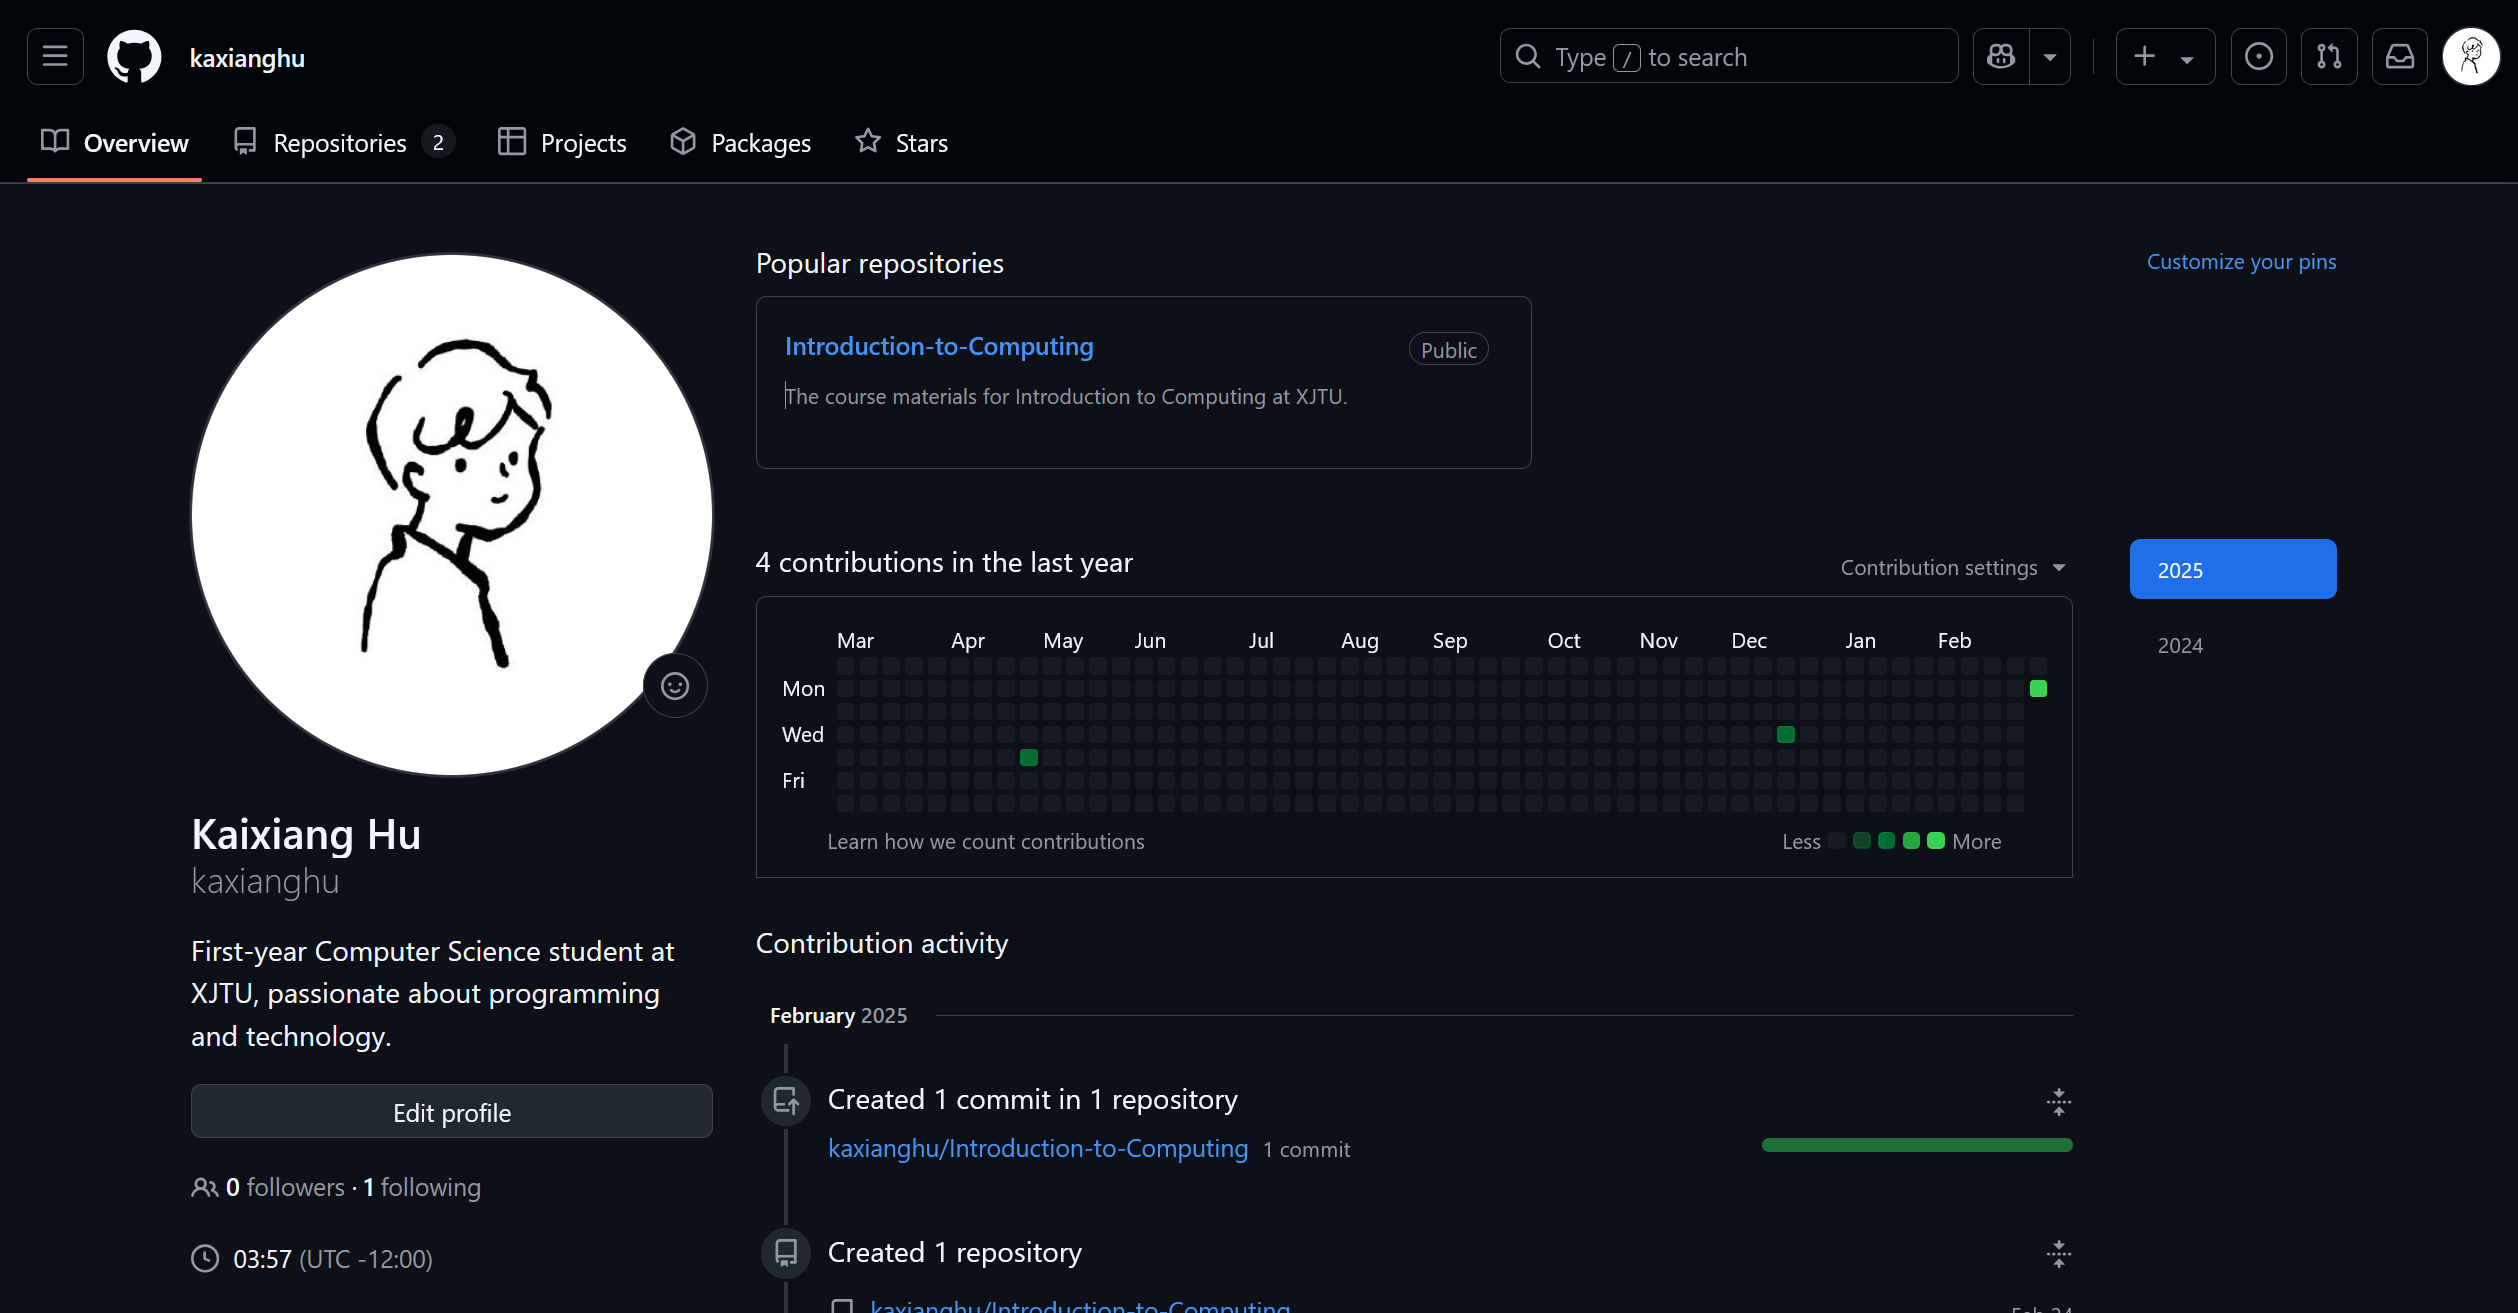
\includegraphics[scale = 0.2]{a.png}
    \end{figure}
\end{solution}

\begin{problem}
    思考题-编程并实现欧拉的信封:我们有编号是1、2、…、n的n封信,装入编号为1、2、…、n的n个信封,要求每封信和信封的编号不同,即1不能装进1,2不能装进 2,3不能装进3……问有多少种装法? 

\end{problem}

\begin{solution}
    已附件
    
    \begin{lstlisting}
def derangement(n):
    if n == 0:
        return 1
    elif n == 1:
        return 0
    else:
        # 递推关系
        return (n - 1) * (derangement(n - 1) + derangement(n - 2))

# 示例:计算n=10时的错排数
n = 10
print(f"n={n}时的错排数为:{derangement(n)}")
    \end{lstlisting}


\end{solution}
\end{document}